\documentclass[12pt]{article}

\usepackage{fullpage}
\usepackage{multicol,multirow}
\usepackage{tabularx}
\usepackage{ulem}
\usepackage[utf8]{inputenc}
\usepackage[russian]{babel}
\usepackage{amsmath}
\usepackage{amssymb}
\usepackage{listing}
\usepackage{graphicx}
\usepackage{color}
\usepackage{titlesec}

\titleformat{\section}
  {\normalfont\Large\bfseries}{\thesection.}{0.3em}{}

\titleformat{\subsection}
  {\normalfont\large\bfseries}{\thesubsection.}{0.3em}{}

\titlespacing{\section}{0pt}{*2}{*2}
\titlespacing{\subsection}{0pt}{*1}{*1}
\titlespacing{\subsubsection}{0pt}{*0}{*0}
\usepackage{listings}
\lstloadlanguages{Lisp}
\lstset{extendedchars=false,
	breaklines=true,
	breakatwhitespace=true,
	keepspaces = true,
	tabsize=2
}
\begin{document}


\section*{Отчет по лабораторной работе №\,5	 
по курсу \guillemotleft  Функциональное программирование\guillemotright}
\begin{flushright}
Студент группы М8О-307 МАИ \textit{Безлуцкая Елизавета}, \textnumero 2 по списку \\
\makebox[7cm]{Контакты: {\tt lizabezlutskaya@gmail.com} \hfill} \\
\makebox[7cm]{Работа выполнена: 30.05.2019 \hfill} \\
\ \\
Преподаватель: Иванов Дмитрий Анатольевич, доц. каф. 806 \\
\makebox[7cm]{Отчет сдан: \hfill} \\
\makebox[7cm]{Итоговая оценка: \hfill} \\
\makebox[7cm]{Подпись преподавателя: \hfill} \\

\end{flushright}

\section{Тема работы}
Обобщённые функции, методы и классы объектов.

\section{Цель работы}
Научиться определять простейшие классы, порождать экземпляры классов, считывать и изменять значения слотов, научиться определять обобщённые функции и методы.

\section{Задание (вариант №36)}
\textbf{\textit{Объемлющий прямоугольник}} для геометрической фигуры - это такой, который

\begin{itemize}
\item полностью заключает в себе фигуру,
\item имеет стороны, параллельные осям координат.
\end{itemize}

Дан экземпляр класса {\tt line} (отрезок), причём концы отрезка могут задаваться как в декартовых (экземплярами {\tt cart}), так и в полярных координатах (экземплярами  {\tt polar}).

Задание: Написать обобщённую функцию и метод, возвращающий список из четырех вершин объемлющего четырёхугольника для отрезка.\\

\begin{lstlisting}
(defgeneric containing-rect (shape))
(defmethod containing-rect ((l line))
  ...)
\end{lstlisting}

\section{Оборудование студента}
Процессор Intel Core i5-3230M 4\,@\,2.6GHz, память: 16Gb, разрядность системы: 64.

\section{Программное обеспечение}
Ubuntu 16.04 LTS, clisp compiler

\section{Идея, метод, алгоритм}
Метод {\tt containing-rect} работает следующим образом:
\begin{itemize}
\setlength{\itemsep}{-1mm} % уменьшает расстояние между элементами списка
\item если отрезок расположен по диагонали ($x_1 \neq x_2$ и $y_1 \neq y_2$), то выводятся вершины $(x_1, y_1), (x_1, y_2), (x_2, y_2), (x_2, y_1)$ (Рис.1)

\item если отрезок расположен по вертикали($x_1 = x_2$), то выводятся кооррдинаты прямоугольника со смещением по $x$ влево и вправо -- $(x_1 - 1, y_1), (x_2 - 1, y_2), (x_2 + 1, y_2), (x_1 + 1, y_1)$(Рис.2)

\item если отрезок расположен по горизонтали($y_1 = y_2$), то выводятся кооррдинаты прямоугольника со смещением по $x$ влево и вправо -- $(x_1, y_1 - 1), (x_2, y_2 - 1), (x_2, y_2 + 1), (x_1, y_1 + 1)$(Рис.3)
\end{itemize}

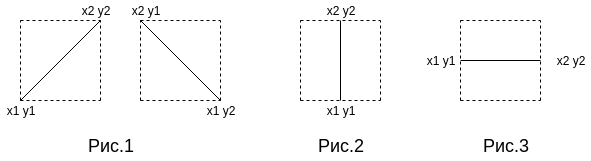
\includegraphics[scale=0.5]{pic.png}

\section{Сценарий выполнения работы}

\section{Распечатка программы и её результаты}

\subsection{Исходный код}

\definecolor{codegreen}{rgb}{0,0.6,0}
\definecolor{codegray}{rgb}{0.5,0.5,0.5}
\definecolor{codepurple}{rgb}{0.58,0,0.82}
\definecolor{backcolour}{rgb}{0.95,0.95,0.92}
 
\lstdefinestyle{mystyle}{
    backgroundcolor=\color{backcolour},   
    commentstyle=\color{codegreen},
    keywordstyle=\color{magenta},
    numberstyle=\tiny\color{codegray},
    stringstyle=\color{codepurple},
    basicstyle=\footnotesize,
    breakatwhitespace=false,         
    breaklines=true,                 
    captionpos=b,                    
    keepspaces=true,                 
    numbers=left,                    
    numbersep=5pt,                  
    showspaces=false,                
    showstringspaces=false,
    showtabs=false,                  
    tabsize=2
}
 
\lstset{style=mystyle} 

\begin{lstlisting}
(defclass line ()
 ((start :initarg :start :accessor line-start)
  (end   :initarg :end   :accessor line-end)))

(defclass cart ()
 ((x :initarg :x :reader cart-x)
  (y :initarg :y :reader cart-y)))

(defmethod print-object ((c cart) stream)
  (format stream "[CART x ~d y ~d]"
          (cart-x c) (cart-y c)))
          
(defclass polar ()
 ((radius :initarg :radius :accessor radius)
  (angle  :initarg :angle  :accessor angle)))

(defmethod cart-x ((p polar))
  (* (radius p) (cos (angle p))))

(defmethod cart-y ((p polar))
  (* (radius p) (sin (angle p))))

(defgeneric containing-rect (shape)
    )

(defmethod containing-rect ((l line))
    (let ((x1 (cart-x (line-start l)))
          (y1 (cart-y (line-start l)))  
          (x2 (cart-x (line-end l)))
          (y2 (cart-y (line-end l))))
        (cond ((= x1 x2) 
                (list (make-instance 'cart :x (1- x1) :y y1)
                      (make-instance 'cart :x (1+ x1) :y y1)
                      (make-instance 'cart :x (1- x2) :y y2)
                      (make-instance 'cart :x (1+ x2) :y y2))
                    )
              ((= y1 y2)
                (list (make-instance 'cart :x x1 :y (1- y1))
                      (make-instance 'cart :x x1 :y (1+ y1))
                      (make-instance 'cart :x x2 :y (1- y2))
                      (make-instance 'cart :x x2 :y (1+ y2))))
              (t 
                (list (make-instance 'cart :x x1 :y y1)
                      (make-instance 'cart :x x1 :y y2)
                      (make-instance 'cart :x x2 :y y2)
                      (make-instance 'cart :x x2 :y y1))))))
\end{lstlisting}


\subsection{Результаты работы}
\begin{lstlisting}             
(print (containing-rect (make-instance 'line
           :start (make-instance 'cart :x 1 :y 3)
           :end (make-instance 'cart :x 4 :y 1))))
([CART x 1 y 3] [CART x 1 y 1] [CART x 4 y 1] [CART x 4 y 3]) 

        
(print (containing-rect (make-instance 'line
           :start (make-instance 'cart :x 2 :y 2)
           :end (make-instance 'cart :x 6 :y 5))))
([CART x 2 y 2] [CART x 2 y 5] [CART x 6 y 5] [CART x 6 y 2]) 


(print (containing-rect (make-instance 'line
           :start (make-instance 'cart :x 2 :y 1)
           :end (make-instance 'cart :x 2 :y 5))))
([CART x 1 y 1] [CART x 3 y 1] [CART x 1 y 5] [CART x 3 y 5])

(print (containing-rect (make-instance 'line
           :start (make-instance 'cart :x 0 :y 1)
           :end (make-instance 'polar :radius 5 :angle (/ pi 4)))))
([CART x 0 y 1] [CART x 0 y 3.5355339059327376221L0]
 [CART x 3.535533905932737622L0 y 3.5355339059327376221L0]
 [CART x 3.535533905932737622L0 y 1]) 
           
\end{lstlisting}

\section{Дневник отладки}
\begin{tabular}{|c|p{5cm}|p{5cm}|p{3cm}|}
\hline
Дата & Событие & Действие по исправлению & Примечание \\
\hline
4.06.2019 & Концы отрезка могут быть заданы и в полярных координатах, не учитывается данный случай & Добавлены методы -- декартовы координаты по полярным & \\
\hline
\end{tabular}

\section{Замечания автора по существу работы}
Замечаний не имею.

\section{Выводы}
В данной лабораторной работе я встретила новую для себя конструкцию -- generic. Считаю, что написание для нее методов в отдельном блоке кода усложняет читаемость программы. Возможно, такое неудобство обосновано для некоторых задач.
\end{document}